\documentclass{article}
\usepackage{tikz}
\usepackage{amsmath}
\usepackage{amssymb}
\usetikzlibrary{automata, positioning, arrows}
\thispagestyle{empty}

\tikzset{
    ->, % makes the edges directed
    >=stealth', % makes the arrow heads bold
    node distance=3cm, % specifies the minimum distance between two nodes. Change if necessary.
    every state/.style={thick, fill=gray!10}, % sets the properties for each ’state’ node
    initial text=$ $, % sets the text that appears on the start arrow
    }

\begin{document}
    \begin{figure}[ht]
        \centering
        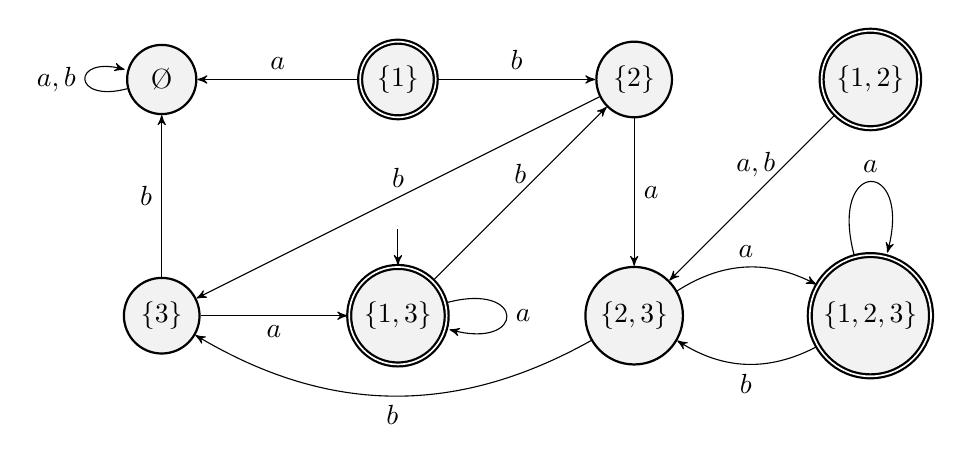
\begin{tikzpicture}

        \node[state] (phi) {$\O$};
\node[state, accepting, right of=phi] (1) {$\{1\}$};
\node[state, right of=1] (2) {$\{2\}$};
\node[state, accepting, right of=2] (12) {$\{1, 2\}$};
\node[state, below of=phi] (3) {$\{3\}$};
\node[state, initial, initial where=above, accepting, right of=3] (13) {$\{1, 3\}$};
\node[state, right of=13] (23) {$\{2, 3\}$};
\node[state, accepting, right of=23] (123) {$\{1, 2, 3\}$};

\draw (phi) edge[loop left] node{$a, b$} (phi)
(1) edge[above] node{$a$} (phi)
(1) edge[above] node{$b$} (2)
(2) edge[right] node{$a$} (23)
(2) edge[above] node{$b$} (3)
(12) edge[above, pos=.3, left=2pt] node{$a, b$} (23)
(3) edge[left] node{$b$} (phi)
(3) edge[below] node{$a$} (13)
(13) edge[loop right] node{$a$} (13)
(13) edge[above] node{$b$} (2)
(23) edge[bend left, above] node{$a$} (123)
(23) edge[bend left, below] node{$b$} (3)
(123) edge[loop above] node{$a$} (123)
(123) edge[bend left, below] node{$b$} (23);

        
        \end{tikzpicture}
    \end{figure}
\end{document}